\section{Method}

This work follows four steps:
\begin{enumerate}
\item Data curation
\item Model training (with hyperparameter optimization)
\item Model validation
\item Model implementation in \Cyclus.
\end{enumerate}
First, the
received data with assembly information is
curated for ease of use in training the model.
Second, we train the neural network using Keras \cite{collet_keras_2015}
and Scikit-learn \cite{pedregosa_scikit-learn_2011},
while using an outer loop to
search for the optimized neural network set of hyperparameters,
such as the number of hidden layers and nodes per layer.
Third, we use the model to predict the U.S. \gls{UNF}
inventory as specified in the \gls{UDB} and compare
\gls{UNF} inventory metrics such as fissile content
and decay heat. Lastly, we implement the trained
model in \Cyclus by developing a facility archetype
that perform depletion calculations with the model.

Codes used to generate and test the neural network
model are all on Github (https://github.com/jbae11/depletion\_rom)
including the pickled neural network model file.

\subsection{Train dataset}

In order to train a depletion model, a large amount of
depletion data is needed.

\subsubsection{Unified Database}
The \gls{UDB} is part of a larger engineering
analysis tool, the \gls{UNF-STANDARDS}, developed
by \gls{ORNL} \cite{peterson_used_2013}. The
database ``provides a comprehensive, controlled
source of \gls{SNF} information, including
dry cask attributes, assembly data, economic attributes,
transportation infrastructure attributes, potential future
facility attributes, and federal government radioactive
waste attributes.

=========================GWEN=========================

We received the database through personal contact
with [i think it's Kaushik Banerjee] [how we got it and stuff]

list of assumptions from the \gls{UNF-STANDARDS} dataset.
\begin{itemize}
    \item UNF database
    \item different assembly geometries?
\end{itemize}

=========================GWENEND=========================

Ideally, the data should be generated with exact same reactor
parameters other than burnup and enrichment, such as geometry or
coolant density. However, since
this is preliminary work to prove potential workflow, we
simply used all the \gls{PWR} datasets in the \gls{UDB}.

\subsection{Data Curation}

We curated the raw \gls{UDB} datasets to generate
a cleaner training set. First we only used the 
\gls{PWR} assemblies since \gls{BWR} \gls{UNF} assembly
calculations can largely vary with void fraction.
We also filtered out the
`very low' enrichment ($\leq$ 1.5) and
burnup ($\leq$ 10,000 MWdth/kg)
assemblies to represent more modern \gls{PWR} \gls{UNF}
assembly range. Figure \ref{fig:enr_bu} shows the
burnup and enrichment distribution of the assemblies in the
\gls{UDB}.


\begin{figure}
    \centering
    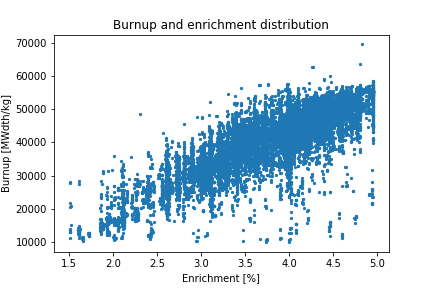
\includegraphics[width=\textwidth]{enr_bu.png}
    \caption{Burnup and enrichment distribution of train
             datasets curated from the \gls{UDB}.}
    \label{fig:enr_bu}
\end{figure}


Also, the SCALE calculation in the \gls{UDB} only tracks 60 isotopes,
and an average of 3.5\% of the \gls{UNF} is not accounted for. We
aggregate the isotopes not accounted for as `other'. Lastly,
we processed the database so that the isotopic compositions are 
represented as \% weight from initial uranium mass, to normalize
the dataset. For every isotope \textit{i}:

\begin{equation}
x_i = \frac{m_i}{M_{initU}}
\end{equation}
where:
\[
x_i = \text{\% weight of depleted assembly}
\]
\[
m_i = \text{mass of isotope in depleted assembly in \gls{UDB}}
\]
\[
M_{initU} = \text{Mass of initial uranium in assembly}
\]


\subsection{Predictive Models for Fuel Depletion}

Isotopic composition of \gls{UNF} is hard to predict due to their
non-linear relationship with fuel parameters. For each
isotope, we plotted isotopic concentration values against
burnup and enrichment to observe the relationship between
burnup, enrichment, and isotope concentration.

We observed that the isotope concentration has varying
relationships with fuel burnup and enrichment.
For example, if the isotope population is mainly determined by
the fission of initial uranium, a linear regression algorithm
can be used to predict the isotope concentration from burnup
(Cs-137 shown in figure \ref{fig:cs_137}).
However, isotopes like plutonium-239 (figure \ref{fig:pu_239}) have multiple, conflicting creation
and destruction terms, making it harder to predict using a
linear regression algorithm. Also, the uranium-235 (figure \ref{fig:u_235}) concentration
depends on both burnup and enrichment, which can make it
hard to predict using a simple linear model.

Due to these complexities, we decided to train an artificial
neural network for our predictive model. We chose
Keras to create and validate the model, as well as scikit-learn
and pandas for data processing and management.

\begin{figure}
    \centering
    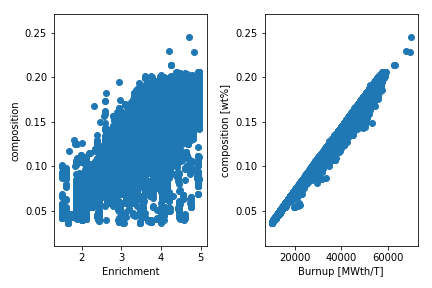
\includegraphics[width=\textwidth]{cs-137_sub.png}
    \caption{Cesium-137 concentration in a \gls{UNF} assembly
             has a linear relationship with assembly burnup.}
    \label{fig:cs_137}
\end{figure}

\begin{figure}
    \centering
    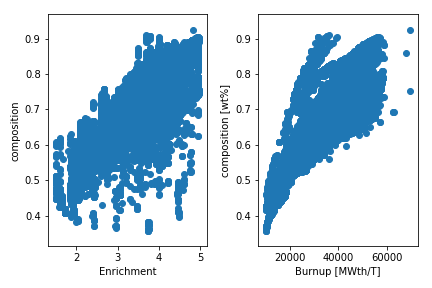
\includegraphics[width=\textwidth]{pu-239_sub.png}
    \caption{Plutonium-239 concentration in a \gls{UNF} assembly
             is not directly proportional to burnup, and is
             not related to initial enrichment.}
    \label{fig:pu_239}
\end{figure}


\begin{figure}
    \centering
    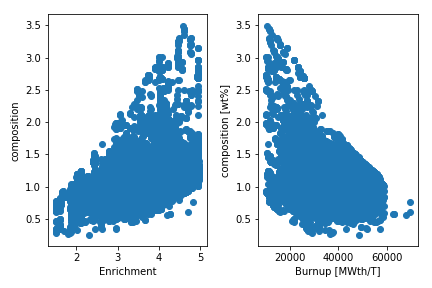
\includegraphics[width=\textwidth]{u-235_sub.png}
    \caption{Uranium-235 concentration in a \gls{UNF} assembly
             somewhat proportional to both enrichment and
             burnup, but is difficult to predict using
             a simple linear regression algorithm.}
    \label{fig:u_235}
\end{figure}


\subsection{Training and Selecting Models}

The input space (feature space) of the model is set to
be burnup (MWdth/kg) and initial enrichment (wt\% U-235).
The output space (target space) of the model is set to
be the concentration of the 60 isotopes in the
depleted assembly.

With the curated dataset, we performed a three-fold
cross validation on the training dataset to find the
best-performing neural network hyperparameter. We
normalized the data using the sklearn MinMaxScaler
so that the range of input and output data is (0,1).

\begin{table}[h]
    \centering
    \begin{tabular}{lr}
        \hline
        Parameter & Values \\
        \hline
        Number of hidden layers & 1, 2, \textbf{3} \\
        Node per hidden layer & 4, 8, \textbf{16}, 32 \\
        Dropout rate & \textbf{0.0}, 0.2, 0.5 \\
        \hline
    \end{tabular}
    \caption{Table of hyperparameters tested
             for neural network model. The bolded
             numbers are values chosen for the final model.}
\end{table}

The model with the smallest average loss value
is selected and is exported as a file using python
pickle, along with the dataset scaling objects, as well as
the list of isotopes. By exporting the trained model
as a file, the model can be used in any python
application by loading the pickled file.


\subsection{Model Testing}

The accuracy of the model is tested by comparing
the model's prediction of \gls{UNF} composition
in three different cases. First, we compare the
isotope-by-isotope prediction error of the model for an
assembly with a specific burnup and enrichment.
Second, we compare the waste characteristics of
an assembly for all assemblies. Third, we compare
the predicted total \gls{PWR} \gls{UNF} inventory with
\gls{UDB}. The metric for error is calculated as
relative error percentage, calculated by:
\begin{equation}
\epsilon = \frac{x_{data} - x_{model}}{x_{data}}
\end{equation}

This metric is to provide fair assessment to errors
in predicting isotopes with minute concentration in \gls{UNF}.
However, it should be noted that a large error percentage in the
prediction of these minute isotopes is mostly because it has been
divided by a small value, not because the absolute error is large.

We compare waste parameters of the \gls{UNF} inventory
such as activity and decay heat, using the
\gls{PyNE} \cite{scopatz_pyne:_2012}. This tool provides
various functions used
in this work, such as decaying material and calculating
the activity and decay heat of the material.

Ideally, the model should be tested against data
that is not part of the training data. However, given
that the purpose of this model is to allow accessible and
quick depletion calculation for
fuel cycle simulations, the model would suffice if
it predicts SCALE results well. In other words, the
goal of the model is to be able to reproduce the
trained dataset without access to this particular dataset.
Again, this work
is to propose a general concept for implementing
rapid depletion models in fuel cycle simulations.
For creating depletion models for other reactor designs,
one would simply change the dataset to a set of depletion
calculations performed for a specific reactor design with
constant operational parameters.


\subsection{Model Application}

The trained model is exported to a file
that can be plugged into external codes. \Cyclus
has a python interface that allows the developer
to design archetypes in python. We developed a reactor
module that behaves the similar to the recipe reactor,
but calculates depleted fuel concentration using the
imported model instead of a recipe. The user can vary
individual assembly burps. The user defines a burnup
and enrichment
matrix for the reactor where the rows are the number
of batches, and the the columns are number of
assemblies in a batch. This reactor module is also
available on Github 
(https://github.com/jbae11/ann\_pwr)

This sort of implementation can be done roughly with
the recipe reactor if the user defines multiple
output recipes. However, the user cannot vary the
burnup or enrichment of the individual assemblies.
Implementing the model will allow the user to vary
burnup and enrichment for individual assemblies, as well
as vary fuel residence time and burnup with reactor
lifetime or simulation time. Such capability will be
useful in simulating \gls{UNF} inventory in the future,
where the burnup of \gls{LWR} fuel will increase
with the advancement of fuel technology.
